% SOURCE: ../../edit-harness/results/merging/RG_gain_law_20260715.json + ../../edit-harness/results/merging/RG_crossterm_alignment_ALL_REFIX20260801.json
% !TEX encoding = UTF-8 Unicode
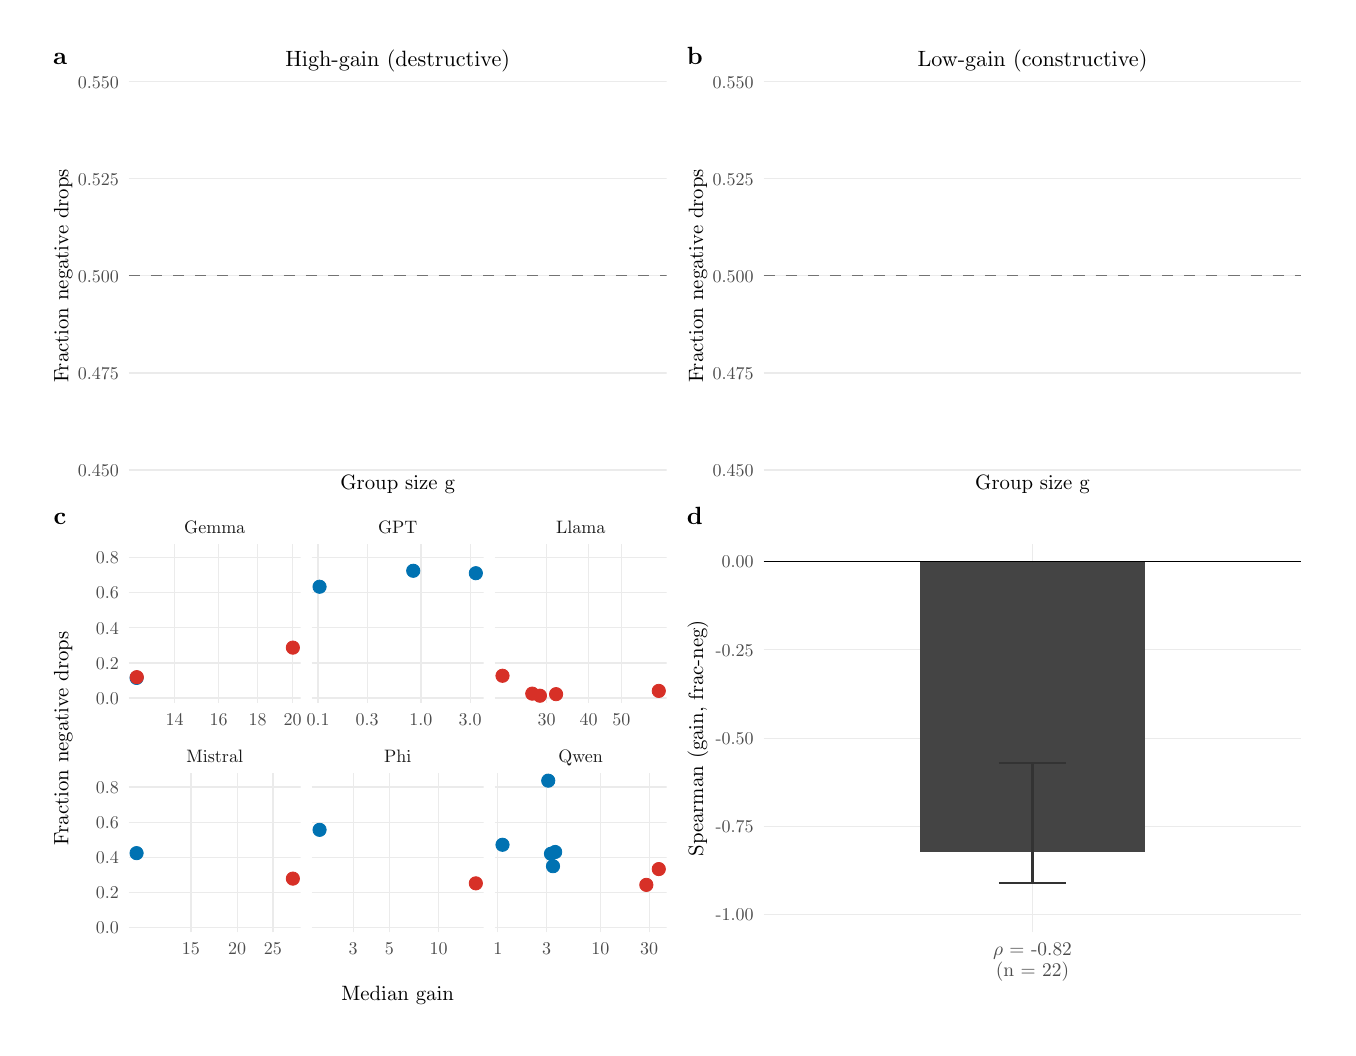
\begin{tikzpicture}[x=1pt,y=1pt]
\definecolor{fillColor}{RGB}{255,255,255}
\path[use as bounding box,fill=fillColor,fill opacity=0.00] (0,0) rectangle (469.75,361.35);
\begin{scope}
\path[clip] (  0.00,  0.00) rectangle (469.75,361.35);
\definecolor{drawColor}{RGB}{255,255,255}
\definecolor{fillColor}{RGB}{255,255,255}

\path[draw=drawColor,line width= 0.6pt,line join=round,line cap=round,fill=fillColor] (  0.00,  0.00) rectangle (469.76,361.35);
\end{scope}
\begin{scope}
\path[clip] (  5.50,189.88) rectangle (234.88,355.85);
\definecolor{fillColor}{RGB}{255,255,255}

\path[fill=fillColor] (  5.50,189.88) rectangle (234.88,355.85);
\end{scope}
\begin{scope}
\path[clip] (234.88,189.88) rectangle (464.26,355.85);
\definecolor{fillColor}{RGB}{255,255,255}

\path[fill=fillColor] (234.88,189.88) rectangle (464.26,355.85);
\end{scope}
\begin{scope}
\path[clip] (  5.50,  5.50) rectangle (234.88,189.88);
\definecolor{fillColor}{RGB}{255,255,255}

\path[fill=fillColor] (  5.50,  5.50) rectangle (234.88,189.88);
\end{scope}
\begin{scope}
\path[clip] (234.88,  5.50) rectangle (464.26,189.88);
\definecolor{fillColor}{RGB}{255,255,255}

\path[fill=fillColor] (234.88,  5.50) rectangle (464.26,189.88);
\end{scope}
\begin{scope}
\path[clip] ( 36.53,201.51) rectangle (230.88,341.79);
\definecolor{drawColor}{gray}{0.92}

\path[draw=drawColor,line width= 0.4pt,line join=round] ( 36.53,201.51) --
	(230.88,201.51);

\path[draw=drawColor,line width= 0.4pt,line join=round] ( 36.53,236.58) --
	(230.88,236.58);

\path[draw=drawColor,line width= 0.4pt,line join=round] ( 36.53,271.65) --
	(230.88,271.65);

\path[draw=drawColor,line width= 0.4pt,line join=round] ( 36.53,306.72) --
	(230.88,306.72);

\path[draw=drawColor,line width= 0.4pt,line join=round] ( 36.53,341.79) --
	(230.88,341.79);
\definecolor{drawColor}{gray}{0.45}

\path[draw=drawColor,line width= 0.3pt,dash pattern=on 4pt off 4pt ,line join=round] ( 36.53,271.65) -- (230.88,271.65);
\end{scope}
\begin{scope}
\path[clip] (  0.00,  0.00) rectangle (469.75,361.35);
\definecolor{drawColor}{gray}{0.30}

\node[text=drawColor,anchor=base east,inner sep=0pt, outer sep=0pt, scale=  0.65] at ( 32.93,199.27) {0.450};

\node[text=drawColor,anchor=base east,inner sep=0pt, outer sep=0pt, scale=  0.65] at ( 32.93,234.34) {0.475};

\node[text=drawColor,anchor=base east,inner sep=0pt, outer sep=0pt, scale=  0.65] at ( 32.93,269.41) {0.500};

\node[text=drawColor,anchor=base east,inner sep=0pt, outer sep=0pt, scale=  0.65] at ( 32.93,304.48) {0.525};

\node[text=drawColor,anchor=base east,inner sep=0pt, outer sep=0pt, scale=  0.65] at ( 32.93,339.55) {0.550};
\end{scope}
\begin{scope}
\path[clip] (  0.00,  0.00) rectangle (469.75,361.35);
\definecolor{drawColor}{RGB}{0,0,0}

\node[text=drawColor,anchor=base,inner sep=0pt, outer sep=0pt, scale=  0.75] at (133.70,194.34) {Group size g};
\end{scope}
\begin{scope}
\path[clip] (  0.00,  0.00) rectangle (469.75,361.35);
\definecolor{drawColor}{RGB}{0,0,0}

\node[text=drawColor,rotate= 90.00,anchor=base,inner sep=0pt, outer sep=0pt, scale=  0.75] at ( 14.67,271.65) {Fraction negative drops};
\end{scope}
\begin{scope}
\path[clip] (  0.00,  0.00) rectangle (469.75,361.35);
\definecolor{drawColor}{RGB}{0,0,0}

\node[text=drawColor,anchor=base,inner sep=0pt, outer sep=0pt, scale=  0.80] at (133.70,347.34) {High-gain (destructive)};
\end{scope}
\begin{scope}
\path[clip] (  0.00,  0.00) rectangle (469.75,361.35);
\definecolor{drawColor}{RGB}{0,0,0}

\node[text=drawColor,anchor=base,inner sep=0pt, outer sep=0pt, scale=  0.90] at ( 11.71,348.14) {\bfseries a};
\end{scope}
\begin{scope}
\path[clip] (265.90,201.51) rectangle (460.25,341.79);
\definecolor{drawColor}{gray}{0.92}

\path[draw=drawColor,line width= 0.4pt,line join=round] (265.90,201.51) --
	(460.25,201.51);

\path[draw=drawColor,line width= 0.4pt,line join=round] (265.90,236.58) --
	(460.25,236.58);

\path[draw=drawColor,line width= 0.4pt,line join=round] (265.90,271.65) --
	(460.25,271.65);

\path[draw=drawColor,line width= 0.4pt,line join=round] (265.90,306.72) --
	(460.25,306.72);

\path[draw=drawColor,line width= 0.4pt,line join=round] (265.90,341.79) --
	(460.25,341.79);
\definecolor{drawColor}{gray}{0.45}

\path[draw=drawColor,line width= 0.3pt,dash pattern=on 4pt off 4pt ,line join=round] (265.90,271.65) -- (460.25,271.65);
\end{scope}
\begin{scope}
\path[clip] (  0.00,  0.00) rectangle (469.75,361.35);
\definecolor{drawColor}{gray}{0.30}

\node[text=drawColor,anchor=base east,inner sep=0pt, outer sep=0pt, scale=  0.65] at (262.30,199.27) {0.450};

\node[text=drawColor,anchor=base east,inner sep=0pt, outer sep=0pt, scale=  0.65] at (262.30,234.34) {0.475};

\node[text=drawColor,anchor=base east,inner sep=0pt, outer sep=0pt, scale=  0.65] at (262.30,269.41) {0.500};

\node[text=drawColor,anchor=base east,inner sep=0pt, outer sep=0pt, scale=  0.65] at (262.30,304.48) {0.525};

\node[text=drawColor,anchor=base east,inner sep=0pt, outer sep=0pt, scale=  0.65] at (262.30,339.55) {0.550};
\end{scope}
\begin{scope}
\path[clip] (  0.00,  0.00) rectangle (469.75,361.35);
\definecolor{drawColor}{RGB}{0,0,0}

\node[text=drawColor,anchor=base,inner sep=0pt, outer sep=0pt, scale=  0.75] at (363.08,194.34) {Group size g};
\end{scope}
\begin{scope}
\path[clip] (  0.00,  0.00) rectangle (469.75,361.35);
\definecolor{drawColor}{RGB}{0,0,0}

\node[text=drawColor,rotate= 90.00,anchor=base,inner sep=0pt, outer sep=0pt, scale=  0.75] at (244.04,271.65) {Fraction negative drops};
\end{scope}
\begin{scope}
\path[clip] (  0.00,  0.00) rectangle (469.75,361.35);
\definecolor{drawColor}{RGB}{0,0,0}

\node[text=drawColor,anchor=base,inner sep=0pt, outer sep=0pt, scale=  0.80] at (363.08,347.34) {Low-gain (constructive)};
\end{scope}
\begin{scope}
\path[clip] (  0.00,  0.00) rectangle (469.75,361.35);
\definecolor{drawColor}{RGB}{0,0,0}

\node[text=drawColor,anchor=base,inner sep=0pt, outer sep=0pt, scale=  0.90] at (241.09,348.14) {\bfseries b};
\end{scope}
\begin{scope}
\path[clip] ( 36.53,117.34) rectangle ( 98.64,174.74);
\definecolor{drawColor}{gray}{0.92}

\path[draw=drawColor,line width= 0.4pt,line join=round] ( 36.53,119.11) --
	( 98.64,119.11);

\path[draw=drawColor,line width= 0.4pt,line join=round] ( 36.53,131.79) --
	( 98.64,131.79);

\path[draw=drawColor,line width= 0.4pt,line join=round] ( 36.53,144.47) --
	( 98.64,144.47);

\path[draw=drawColor,line width= 0.4pt,line join=round] ( 36.53,157.15) --
	( 98.64,157.15);

\path[draw=drawColor,line width= 0.4pt,line join=round] ( 36.53,169.83) --
	( 98.64,169.83);

\path[draw=drawColor,line width= 0.4pt,line join=round] ( 53.06,117.34) --
	( 53.06,174.74);

\path[draw=drawColor,line width= 0.4pt,line join=round] ( 69.03,117.34) --
	( 69.03,174.74);

\path[draw=drawColor,line width= 0.4pt,line join=round] ( 83.12,117.34) --
	( 83.12,174.74);

\path[draw=drawColor,line width= 0.4pt,line join=round] ( 95.72,117.34) --
	( 95.72,174.74);
\definecolor{drawColor}{RGB}{215,48,39}
\definecolor{fillColor}{RGB}{215,48,39}

\path[draw=drawColor,line width= 0.3pt,line join=round,line cap=round,fill=fillColor] ( 95.82,137.33) circle (  2.40);
\definecolor{drawColor}{RGB}{0,114,178}
\definecolor{fillColor}{RGB}{0,114,178}

\path[draw=drawColor,line width= 0.3pt,line join=round,line cap=round,fill=fillColor] ( 39.35,126.38) circle (  2.40);
\definecolor{drawColor}{RGB}{215,48,39}
\definecolor{fillColor}{RGB}{215,48,39}

\path[draw=drawColor,line width= 0.3pt,line join=round,line cap=round,fill=fillColor] ( 39.43,126.66) circle (  2.40);
\end{scope}
\begin{scope}
\path[clip] ( 36.53, 34.47) rectangle ( 98.64, 91.86);
\definecolor{drawColor}{gray}{0.92}

\path[draw=drawColor,line width= 0.4pt,line join=round] ( 36.53, 36.23) --
	( 98.64, 36.23);

\path[draw=drawColor,line width= 0.4pt,line join=round] ( 36.53, 48.91) --
	( 98.64, 48.91);

\path[draw=drawColor,line width= 0.4pt,line join=round] ( 36.53, 61.59) --
	( 98.64, 61.59);

\path[draw=drawColor,line width= 0.4pt,line join=round] ( 36.53, 74.27) --
	( 98.64, 74.27);

\path[draw=drawColor,line width= 0.4pt,line join=round] ( 36.53, 86.95) --
	( 98.64, 86.95);

\path[draw=drawColor,line width= 0.4pt,line join=round] ( 59.01, 34.47) --
	( 59.01, 91.86);

\path[draw=drawColor,line width= 0.4pt,line join=round] ( 75.70, 34.47) --
	( 75.70, 91.86);

\path[draw=drawColor,line width= 0.4pt,line join=round] ( 88.64, 34.47) --
	( 88.64, 91.86);
\definecolor{drawColor}{RGB}{215,48,39}
\definecolor{fillColor}{RGB}{215,48,39}

\path[draw=drawColor,line width= 0.3pt,line join=round,line cap=round,fill=fillColor] ( 95.82, 53.86) circle (  2.40);
\definecolor{drawColor}{RGB}{0,114,178}
\definecolor{fillColor}{RGB}{0,114,178}

\path[draw=drawColor,line width= 0.3pt,line join=round,line cap=round,fill=fillColor] ( 39.35, 63.07) circle (  2.40);
\end{scope}
\begin{scope}
\path[clip] (102.64,117.34) rectangle (164.76,174.74);
\definecolor{drawColor}{gray}{0.92}

\path[draw=drawColor,line width= 0.4pt,line join=round] (102.64,119.11) --
	(164.76,119.11);

\path[draw=drawColor,line width= 0.4pt,line join=round] (102.64,131.79) --
	(164.76,131.79);

\path[draw=drawColor,line width= 0.4pt,line join=round] (102.64,144.47) --
	(164.76,144.47);

\path[draw=drawColor,line width= 0.4pt,line join=round] (102.64,157.15) --
	(164.76,157.15);

\path[draw=drawColor,line width= 0.4pt,line join=round] (102.64,169.83) --
	(164.76,169.83);

\path[draw=drawColor,line width= 0.4pt,line join=round] (104.91,117.34) --
	(104.91,174.74);

\path[draw=drawColor,line width= 0.4pt,line join=round] (122.66,117.34) --
	(122.66,174.74);

\path[draw=drawColor,line width= 0.4pt,line join=round] (142.12,117.34) --
	(142.12,174.74);

\path[draw=drawColor,line width= 0.4pt,line join=round] (159.87,117.34) --
	(159.87,174.74);
\definecolor{drawColor}{RGB}{0,114,178}
\definecolor{fillColor}{RGB}{0,114,178}

\path[draw=drawColor,line width= 0.3pt,line join=round,line cap=round,fill=fillColor] (105.47,159.33) circle (  2.40);

\path[draw=drawColor,line width= 0.3pt,line join=round,line cap=round,fill=fillColor] (161.94,164.22) circle (  2.40);

\path[draw=drawColor,line width= 0.3pt,line join=round,line cap=round,fill=fillColor] (139.32,165.10) circle (  2.40);
\end{scope}
\begin{scope}
\path[clip] (102.64, 34.47) rectangle (164.76, 91.86);
\definecolor{drawColor}{gray}{0.92}

\path[draw=drawColor,line width= 0.4pt,line join=round] (102.64, 36.23) --
	(164.76, 36.23);

\path[draw=drawColor,line width= 0.4pt,line join=round] (102.64, 48.91) --
	(164.76, 48.91);

\path[draw=drawColor,line width= 0.4pt,line join=round] (102.64, 61.59) --
	(164.76, 61.59);

\path[draw=drawColor,line width= 0.4pt,line join=round] (102.64, 74.27) --
	(164.76, 74.27);

\path[draw=drawColor,line width= 0.4pt,line join=round] (102.64, 86.95) --
	(164.76, 86.95);

\path[draw=drawColor,line width= 0.4pt,line join=round] (117.62, 34.47) --
	(117.62, 91.86);

\path[draw=drawColor,line width= 0.4pt,line join=round] (130.70, 34.47) --
	(130.70, 91.86);

\path[draw=drawColor,line width= 0.4pt,line join=round] (148.46, 34.47) --
	(148.46, 91.86);
\definecolor{drawColor}{RGB}{215,48,39}
\definecolor{fillColor}{RGB}{215,48,39}

\path[draw=drawColor,line width= 0.3pt,line join=round,line cap=round,fill=fillColor] (161.94, 52.15) circle (  2.40);
\definecolor{drawColor}{RGB}{0,114,178}
\definecolor{fillColor}{RGB}{0,114,178}

\path[draw=drawColor,line width= 0.3pt,line join=round,line cap=round,fill=fillColor] (105.47, 71.49) circle (  2.40);
\end{scope}
\begin{scope}
\path[clip] (168.76,117.34) rectangle (230.88,174.74);
\definecolor{drawColor}{gray}{0.92}

\path[draw=drawColor,line width= 0.4pt,line join=round] (168.76,119.11) --
	(230.88,119.11);

\path[draw=drawColor,line width= 0.4pt,line join=round] (168.76,131.79) --
	(230.88,131.79);

\path[draw=drawColor,line width= 0.4pt,line join=round] (168.76,144.47) --
	(230.88,144.47);

\path[draw=drawColor,line width= 0.4pt,line join=round] (168.76,157.15) --
	(230.88,157.15);

\path[draw=drawColor,line width= 0.4pt,line join=round] (168.76,169.83) --
	(230.88,169.83);

\path[draw=drawColor,line width= 0.4pt,line join=round] (187.51,117.34) --
	(187.51,174.74);

\path[draw=drawColor,line width= 0.4pt,line join=round] (202.74,117.34) --
	(202.74,174.74);

\path[draw=drawColor,line width= 0.4pt,line join=round] (214.55,117.34) --
	(214.55,174.74);
\definecolor{drawColor}{RGB}{215,48,39}
\definecolor{fillColor}{RGB}{215,48,39}

\path[draw=drawColor,line width= 0.3pt,line join=round,line cap=round,fill=fillColor] (171.58,127.16) circle (  2.40);

\path[draw=drawColor,line width= 0.3pt,line join=round,line cap=round,fill=fillColor] (182.33,120.70) circle (  2.40);

\path[draw=drawColor,line width= 0.3pt,line join=round,line cap=round,fill=fillColor] (185.10,119.95) circle (  2.40);

\path[draw=drawColor,line width= 0.3pt,line join=round,line cap=round,fill=fillColor] (228.05,121.69) circle (  2.40);

\path[draw=drawColor,line width= 0.3pt,line join=round,line cap=round,fill=fillColor] (190.94,120.51) circle (  2.40);
\end{scope}
\begin{scope}
\path[clip] (168.76, 34.47) rectangle (230.88, 91.86);
\definecolor{drawColor}{gray}{0.92}

\path[draw=drawColor,line width= 0.4pt,line join=round] (168.76, 36.23) --
	(230.88, 36.23);

\path[draw=drawColor,line width= 0.4pt,line join=round] (168.76, 48.91) --
	(230.88, 48.91);

\path[draw=drawColor,line width= 0.4pt,line join=round] (168.76, 61.59) --
	(230.88, 61.59);

\path[draw=drawColor,line width= 0.4pt,line join=round] (168.76, 74.27) --
	(230.88, 74.27);

\path[draw=drawColor,line width= 0.4pt,line join=round] (168.76, 86.95) --
	(230.88, 86.95);

\path[draw=drawColor,line width= 0.4pt,line join=round] (169.90, 34.47) --
	(169.90, 91.86);

\path[draw=drawColor,line width= 0.4pt,line join=round] (187.56, 34.47) --
	(187.56, 91.86);

\path[draw=drawColor,line width= 0.4pt,line join=round] (206.92, 34.47) --
	(206.92, 91.86);

\path[draw=drawColor,line width= 0.4pt,line join=round] (224.58, 34.47) --
	(224.58, 91.86);
\definecolor{drawColor}{RGB}{215,48,39}
\definecolor{fillColor}{RGB}{215,48,39}

\path[draw=drawColor,line width= 0.3pt,line join=round,line cap=round,fill=fillColor] (223.55, 51.60) circle (  2.40);
\definecolor{drawColor}{RGB}{0,114,178}
\definecolor{fillColor}{RGB}{0,114,178}

\path[draw=drawColor,line width= 0.3pt,line join=round,line cap=round,fill=fillColor] (189.09, 62.84) circle (  2.40);

\path[draw=drawColor,line width= 0.3pt,line join=round,line cap=round,fill=fillColor] (171.58, 66.09) circle (  2.40);

\path[draw=drawColor,line width= 0.3pt,line join=round,line cap=round,fill=fillColor] (188.10, 89.25) circle (  2.40);
\definecolor{drawColor}{RGB}{215,48,39}
\definecolor{fillColor}{RGB}{215,48,39}

\path[draw=drawColor,line width= 0.3pt,line join=round,line cap=round,fill=fillColor] (228.05, 57.31) circle (  2.40);
\definecolor{drawColor}{RGB}{0,114,178}
\definecolor{fillColor}{RGB}{0,114,178}

\path[draw=drawColor,line width= 0.3pt,line join=round,line cap=round,fill=fillColor] (190.61, 63.48) circle (  2.40);

\path[draw=drawColor,line width= 0.3pt,line join=round,line cap=round,fill=fillColor] (189.82, 58.35) circle (  2.40);
\end{scope}
\begin{scope}
\path[clip] ( 36.53, 91.86) rectangle ( 98.64,104.00);
\definecolor{drawColor}{gray}{0.10}

\node[text=drawColor,anchor=base,inner sep=0pt, outer sep=0pt, scale=  0.65] at ( 67.58, 95.70) {Mistral};
\end{scope}
\begin{scope}
\path[clip] (102.64, 91.86) rectangle (164.76,104.00);
\definecolor{drawColor}{gray}{0.10}

\node[text=drawColor,anchor=base,inner sep=0pt, outer sep=0pt, scale=  0.65] at (133.70, 95.70) {Phi};
\end{scope}
\begin{scope}
\path[clip] (168.76, 91.86) rectangle (230.88,104.00);
\definecolor{drawColor}{gray}{0.10}

\node[text=drawColor,anchor=base,inner sep=0pt, outer sep=0pt, scale=  0.65] at (199.82, 95.70) {Qwen};
\end{scope}
\begin{scope}
\path[clip] (  0.00,  0.00) rectangle (469.75,361.35);
\definecolor{drawColor}{gray}{0.30}

\node[text=drawColor,anchor=base,inner sep=0pt, outer sep=0pt, scale=  0.65] at ( 53.06,109.27) {14};

\node[text=drawColor,anchor=base,inner sep=0pt, outer sep=0pt, scale=  0.65] at ( 69.03,109.27) {16};

\node[text=drawColor,anchor=base,inner sep=0pt, outer sep=0pt, scale=  0.65] at ( 83.12,109.27) {18};

\node[text=drawColor,anchor=base,inner sep=0pt, outer sep=0pt, scale=  0.65] at ( 95.72,109.27) {20};
\end{scope}
\begin{scope}
\path[clip] (  0.00,  0.00) rectangle (469.75,361.35);
\definecolor{drawColor}{gray}{0.30}

\node[text=drawColor,anchor=base,inner sep=0pt, outer sep=0pt, scale=  0.65] at (104.91,109.27) {0.1};

\node[text=drawColor,anchor=base,inner sep=0pt, outer sep=0pt, scale=  0.65] at (122.66,109.27) {0.3};

\node[text=drawColor,anchor=base,inner sep=0pt, outer sep=0pt, scale=  0.65] at (142.12,109.27) {1.0};

\node[text=drawColor,anchor=base,inner sep=0pt, outer sep=0pt, scale=  0.65] at (159.87,109.27) {3.0};
\end{scope}
\begin{scope}
\path[clip] (  0.00,  0.00) rectangle (469.75,361.35);
\definecolor{drawColor}{gray}{0.30}

\node[text=drawColor,anchor=base,inner sep=0pt, outer sep=0pt, scale=  0.65] at (187.51,109.27) {30};

\node[text=drawColor,anchor=base,inner sep=0pt, outer sep=0pt, scale=  0.65] at (202.74,109.27) {40};

\node[text=drawColor,anchor=base,inner sep=0pt, outer sep=0pt, scale=  0.65] at (214.55,109.27) {50};
\end{scope}
\begin{scope}
\path[clip] ( 36.53,174.74) rectangle ( 98.64,186.88);
\definecolor{drawColor}{gray}{0.10}

\node[text=drawColor,anchor=base,inner sep=0pt, outer sep=0pt, scale=  0.65] at ( 67.58,178.58) {Gemma};
\end{scope}
\begin{scope}
\path[clip] (102.64,174.74) rectangle (164.76,186.88);
\definecolor{drawColor}{gray}{0.10}

\node[text=drawColor,anchor=base,inner sep=0pt, outer sep=0pt, scale=  0.65] at (133.70,178.58) {GPT};
\end{scope}
\begin{scope}
\path[clip] (168.76,174.74) rectangle (230.88,186.88);
\definecolor{drawColor}{gray}{0.10}

\node[text=drawColor,anchor=base,inner sep=0pt, outer sep=0pt, scale=  0.65] at (199.82,178.58) {Llama};
\end{scope}
\begin{scope}
\path[clip] (  0.00,  0.00) rectangle (469.75,361.35);
\definecolor{drawColor}{gray}{0.30}

\node[text=drawColor,anchor=base,inner sep=0pt, outer sep=0pt, scale=  0.65] at ( 59.01, 26.39) {15};

\node[text=drawColor,anchor=base,inner sep=0pt, outer sep=0pt, scale=  0.65] at ( 75.70, 26.39) {20};

\node[text=drawColor,anchor=base,inner sep=0pt, outer sep=0pt, scale=  0.65] at ( 88.64, 26.39) {25};
\end{scope}
\begin{scope}
\path[clip] (  0.00,  0.00) rectangle (469.75,361.35);
\definecolor{drawColor}{gray}{0.30}

\node[text=drawColor,anchor=base,inner sep=0pt, outer sep=0pt, scale=  0.65] at (117.62, 26.39) {3};

\node[text=drawColor,anchor=base,inner sep=0pt, outer sep=0pt, scale=  0.65] at (130.70, 26.39) {5};

\node[text=drawColor,anchor=base,inner sep=0pt, outer sep=0pt, scale=  0.65] at (148.46, 26.39) {10};
\end{scope}
\begin{scope}
\path[clip] (  0.00,  0.00) rectangle (469.75,361.35);
\definecolor{drawColor}{gray}{0.30}

\node[text=drawColor,anchor=base,inner sep=0pt, outer sep=0pt, scale=  0.65] at (169.90, 26.39) {1};

\node[text=drawColor,anchor=base,inner sep=0pt, outer sep=0pt, scale=  0.65] at (187.56, 26.39) {3};

\node[text=drawColor,anchor=base,inner sep=0pt, outer sep=0pt, scale=  0.65] at (206.92, 26.39) {10};

\node[text=drawColor,anchor=base,inner sep=0pt, outer sep=0pt, scale=  0.65] at (224.58, 26.39) {30};
\end{scope}
\begin{scope}
\path[clip] (  0.00,  0.00) rectangle (469.75,361.35);
\definecolor{drawColor}{gray}{0.30}

\node[text=drawColor,anchor=base east,inner sep=0pt, outer sep=0pt, scale=  0.65] at ( 32.93,116.87) {0.0};

\node[text=drawColor,anchor=base east,inner sep=0pt, outer sep=0pt, scale=  0.65] at ( 32.93,129.55) {0.2};

\node[text=drawColor,anchor=base east,inner sep=0pt, outer sep=0pt, scale=  0.65] at ( 32.93,142.23) {0.4};

\node[text=drawColor,anchor=base east,inner sep=0pt, outer sep=0pt, scale=  0.65] at ( 32.93,154.91) {0.6};

\node[text=drawColor,anchor=base east,inner sep=0pt, outer sep=0pt, scale=  0.65] at ( 32.93,167.59) {0.8};
\end{scope}
\begin{scope}
\path[clip] (  0.00,  0.00) rectangle (469.75,361.35);
\definecolor{drawColor}{gray}{0.30}

\node[text=drawColor,anchor=base east,inner sep=0pt, outer sep=0pt, scale=  0.65] at ( 32.93, 33.99) {0.0};

\node[text=drawColor,anchor=base east,inner sep=0pt, outer sep=0pt, scale=  0.65] at ( 32.93, 46.67) {0.2};

\node[text=drawColor,anchor=base east,inner sep=0pt, outer sep=0pt, scale=  0.65] at ( 32.93, 59.35) {0.4};

\node[text=drawColor,anchor=base east,inner sep=0pt, outer sep=0pt, scale=  0.65] at ( 32.93, 72.03) {0.6};

\node[text=drawColor,anchor=base east,inner sep=0pt, outer sep=0pt, scale=  0.65] at ( 32.93, 84.72) {0.8};
\end{scope}
\begin{scope}
\path[clip] (  0.00,  0.00) rectangle (469.75,361.35);
\definecolor{drawColor}{RGB}{0,0,0}

\node[text=drawColor,anchor=base,inner sep=0pt, outer sep=0pt, scale=  0.75] at (133.70,  9.96) {Median gain};
\end{scope}
\begin{scope}
\path[clip] (  0.00,  0.00) rectangle (469.75,361.35);
\definecolor{drawColor}{RGB}{0,0,0}

\node[text=drawColor,rotate= 90.00,anchor=base,inner sep=0pt, outer sep=0pt, scale=  0.75] at ( 14.67,104.60) {Fraction negative drops};
\end{scope}
\begin{scope}
\path[clip] (  0.00,  0.00) rectangle (469.75,361.35);
\definecolor{drawColor}{RGB}{0,0,0}

\node[text=drawColor,anchor=base,inner sep=0pt, outer sep=0pt, scale=  0.90] at ( 11.71,181.99) {\bfseries c};
\end{scope}
\begin{scope}
\path[clip] (265.90, 34.47) rectangle (460.25,174.74);
\definecolor{drawColor}{gray}{0.92}

\path[draw=drawColor,line width= 0.4pt,line join=round] (265.90, 40.84) --
	(460.25, 40.84);

\path[draw=drawColor,line width= 0.4pt,line join=round] (265.90, 72.72) --
	(460.25, 72.72);

\path[draw=drawColor,line width= 0.4pt,line join=round] (265.90,104.60) --
	(460.25,104.60);

\path[draw=drawColor,line width= 0.4pt,line join=round] (265.90,136.49) --
	(460.25,136.49);

\path[draw=drawColor,line width= 0.4pt,line join=round] (265.90,168.37) --
	(460.25,168.37);

\path[draw=drawColor,line width= 0.4pt,line join=round] (363.08, 34.47) --
	(363.08,174.74);
\definecolor{fillColor}{RGB}{68,68,68}

\path[fill=fillColor] (322.59, 63.59) rectangle (403.57,168.37);
\definecolor{drawColor}{gray}{0.20}

\path[draw=drawColor,line width= 0.8pt,line join=round] (350.93, 95.68) --
	(375.23, 95.68);

\path[draw=drawColor,line width= 0.8pt,line join=round] (363.08, 95.68) --
	(363.08, 52.32);

\path[draw=drawColor,line width= 0.8pt,line join=round] (350.93, 52.32) --
	(375.23, 52.32);
\definecolor{drawColor}{RGB}{0,0,0}

\path[draw=drawColor,line width= 0.3pt,line join=round] (265.90,168.37) -- (460.25,168.37);
\end{scope}
\begin{scope}
\path[clip] (  0.00,  0.00) rectangle (469.75,361.35);
\definecolor{drawColor}{gray}{0.30}

\node[text=drawColor,anchor=base east,inner sep=0pt, outer sep=0pt, scale=  0.65] at (262.30, 38.60) {-1.00};

\node[text=drawColor,anchor=base east,inner sep=0pt, outer sep=0pt, scale=  0.65] at (262.30, 70.48) {-0.75};

\node[text=drawColor,anchor=base east,inner sep=0pt, outer sep=0pt, scale=  0.65] at (262.30,102.37) {-0.50};

\node[text=drawColor,anchor=base east,inner sep=0pt, outer sep=0pt, scale=  0.65] at (262.30,134.25) {-0.25};

\node[text=drawColor,anchor=base east,inner sep=0pt, outer sep=0pt, scale=  0.65] at (262.30,166.13) {0.00};
\end{scope}
\begin{scope}
\path[clip] (  0.00,  0.00) rectangle (469.75,361.35);
\definecolor{drawColor}{gray}{0.30}

\node[text=drawColor,anchor=base,inner sep=0pt, outer sep=0pt, scale=  0.70] at (363.08, 26.04) {$\rho$ = -0.82};

\node[text=drawColor,anchor=base,inner sep=0pt, outer sep=0pt, scale=  0.70] at (363.08, 18.48) {(n = 22)};
\end{scope}
\begin{scope}
\path[clip] (  0.00,  0.00) rectangle (469.75,361.35);
\definecolor{drawColor}{RGB}{0,0,0}

\node[text=drawColor,rotate= 90.00,anchor=base,inner sep=0pt, outer sep=0pt, scale=  0.75] at (244.04,104.60) {Spearman (gain, frac-neg)};
\end{scope}
\begin{scope}
\path[clip] (  0.00,  0.00) rectangle (469.75,361.35);
\definecolor{drawColor}{RGB}{0,0,0}

\node[text=drawColor,anchor=base,inner sep=0pt, outer sep=0pt, scale=  0.90] at (241.09,181.99) {\bfseries d};
\end{scope}
\end{tikzpicture}
